\section{Result 1}
Assessing the relationship between student benchmarks and CSC1015F grades for all students requires a join of the demographic (FU) data with Grade data. For this analysis the \textit{nETL} configuration (see \ref{netl-run1-config}) specifies two source CSVs: ``FU-CombinedGrades-2016Reg.csv'' (FU data) and ``CombinedGrades.csv'' (Grade data). \textit{nETL} execution is discusses in terms of each CSV source below, followed by a description of the configuration to run the CouchDB MapReduce calculation and retrieval of the result. The Map function and List function as configured for couchDB can also be found in the appendix; see \ref{result-1-map} and \ref{result-1-list} respectively.

Runtime statistics as shown in Figure \ref{performance-analysis} show that both nETL and CouchDB handle this analysis with ease, with a minimal CouchDB footprint (both for the data file and index file), and very quick running times for the nETL tasks and CouchDB index calculation.

\subsection*{\textit{nETL} Grade data configuration}
\begin{itemize}
    \item Batches of 10 000 lines are extracted iteratively (and sequentially) as an array of lines
    \item Within each batch, each line is converted to a JSON object, transforming the batch into an array of objects. These objects each have the following fields: ``DownloadedDate'', ``RegAcadYear'', ``RegTerm'', ``anonIDnew'', ``RegProgram'', ``RegCareer'', ``Degree'', ``DegreeDescr'', ``Subject'', ``Catalog.'', ``Course'', ``CourseSuffix'', ``Session'', ``Percent'', ``Symbol'', ``UnitsTaken'', ``CourseID'', ``CourseDescr'', ``CourseCareer'', ``Faculty'', ``Dept'', ``MaximumCrseUnits'', ``CourseCount'', ``CourseLevel'', ``CESM'', ``Sub-CESM''
    \item The array of objects is filtered via whitelising objects on two fields: 1) ``RegCareer'' - only the value ``UGRD'' is considered. 2) ``Course'' - only the value ``CSC1015F'' is considered. As a result the resultant array (the batch) contains a reduced number of objects
    \item A field is added to each object in the batch (``type\_'') and give the value ``courseGrade'' (this allows for logically tracking the type of entity that each document represents)
    \item Superfluous object fields are removed via a whitelisting process, resulting in a batch (an array) of objects with the fields: ``type\_'', ``Course'', ``RegAcadYear'', ``anonIDnew'', ``Percent''
    \item Each batch is loaded into CouchDB using the \textit{\_bulk\_docs} endpoint (as discussed previously), and the next batch is extracted on a success message from CouchDB
\end{itemize}

\subsection*{\textit{nETL} FU data configuration}
\begin{itemize}
    \item Batches of 10 000 lines are extracted iteratively (and sequentially) as an array of lines
    \item Within each batch, each line is converted to a JSON object, transforming the batch into an array of objects. These objects each have the following fields: ``anonIDnew'', ``Career'', ``Citizenship Residency'', ``SA School'', ``Eng Grd12 Fin Rslt'', ``Math Grd12 Fin Rslt'', ``Mth Lit Grd12 Fin Rslt'', ``Adv Mth Grd12 Fin Rslt'', ``Phy Sci Grd12 Fin Rslt'', ``NBT AL Score'', ``NBT QL Score'', ``NBT Math Score'', ``RegAcadYear''
    \item The array of objects is filtered via whitelising objects on three fields: 1) ``Career'' - the values ``UGRD'', ``First Year'', ``Second Year'', and ``Third Year'' are considered. 2) ``Citizenship Residency'' - the values ``SA Citizen'', ``Permanent Resident'', ``C'', ``P'' are considered. 3) ``anonIDnew'' - a list of student Ids for students that attended CSC1015F at any time during their undergraduate careers. This list was prepared manually for the purposes of this project
    \item A field is added to each object in the batch (``type\_'') and give the value ``demographic'' (this data is actually a subset of general demographic data)
    \item Superfluous object fields are removed via a whitelisting process, resulting in a batch (an array) of objects with the fields: type\_'', ``anonIDnew'', ``Eng Grd12 Fin Rslt'', ``Math Grd12 Fin Rslt'', ``Mth Lit Grd12 Fin Rslt'', ``Adv Mth Grd12 Fin Rslt'', ``Phy Sci Grd12 Fin Rslt'', ``NBT AL Score'', ``NBT QL Score'', ``NBT Math Score'', ``RegAcadYear''
    \item Each batch is loaded into CouchDB using the \textit{\_bulk\_docs} and the next batch extracted
\end{itemize}

\subsection*{The MapReduce function}
To maintain the resolution that exists within the Grade data, that is; \textit{results of a particular student in a particular year for a particular course}, the map function is configured to emit a tuple - [studentID, courseCode, year] - for keys. Compound keys are discussed previously, but effectively they allow for a configurable level of grouping values output by the map task. The benefit of emitting compound keys as keys is that different groupings can be taken without recalculation of indexes, but only `exact' grouping was used in this project. Specification for the value output is also a tuple of the form [course \%, Gr12 English \%, Gr12 science \%, Gr12 Math \%, Gr 12 Math Lit \%, Gr12 Adv Math \%, NBT AL \%, NBT QL \%, NBT Math \%].

The map function for this analysis is included in  the appendix (see \ref{result-1-map}). Each document passed to the map function is treated according to the logic shown in the activity diagram in Figure \ref{result-1-map-fn}. That is, a document's type is checked. If the document is of type ``courseGrade'', the Percent field of the doc is retrieved and normalized to a number using the logic described in Table \ref{tbl-sakai-grades-percent}. The year of the course and the student ID is also retrieved from the document, and then the function emits a key:value pair of the form \textit{[student ID, course, year]: [Percent, 0, 0, 0, 0, 0, 0, 0, 0]}. If the document is of type ``demographic'', then all the benchmarks are retrieved from the document. Benchmarks are normalized to a number according to the logic shown in Table  \ref{tbl-fu-grades-percent}, and then the function emits a key:value pair of the form \textit{[student Id, `a', 1]: [0, all the benchmark \%s]}. Map output is reduced using the built-in \textit{\_stats} function, which doesn't require user configuration.

\begin{figure}[ht]
    \centering
    \begin{mdframed}
        \centering
        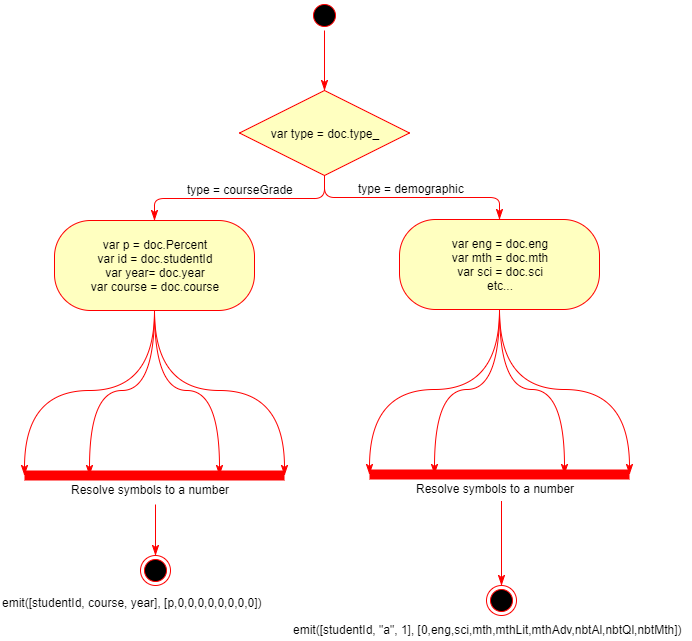
\includegraphics[scale=0.35]{./resources/figures/activity-diagram-1.png}
    \end{mdframed}
    \caption[Result 1 Map function]{\textbf{Figure \ref{result-1-map-fn}: Activity diagram showing logic Map function logic for Results 1 \& 2.} This logic is applied to every document during index calculation (excluding documents with an \_id of ``\_design/*'').}
    \label{result-1-map-fn}
\end{figure}

\subsection*{The List function}
The list function is used to iterate over the results of the MapReduce view, and transform the JSON structure of the view return into a CSV. The list function is included in the appendix (see \ref{result-1-list}). The logic is fairly straight forward; The list function is called via HTTP, specifying the view in the URL, along with the options to group map output by key (at exact level) and to use the reduced result set. The List function first emits a row of headers, as defined in the function itself, and then iterates over the keys in the MapReduce index. For each key, the List function emits a string of comma separated values followed by a newline char according to the RFC 4180 specification. This allows for CSV's to be created and downloaded incrementally allowing for iteration over huge MapReduce indexes.

As mentioned previously List functions are likely to become deprecated in CouchDB. As such it would be better practice to replicate the logic of the List function in a node.js (or alternative) application. If this were to be done, the logic involved in producing a CSV from the MapReduce results would remain the same.
